\documentclass[a4paper,
fontsize=11pt,
%headings=small,
oneside,
numbers=noperiodatend,
parskip=half-,
bibliography=totoc,
final
]{scrartcl}

\usepackage[babel]{csquotes}
\usepackage{synttree}
\usepackage{graphicx}
\setkeys{Gin}{width=.6\textwidth} %default pics size

\graphicspath{{./plots/}}
\usepackage[english]{babel}
\usepackage[T1]{fontenc}
%\usepackage{amsmath}
\usepackage[utf8x]{inputenc}
\usepackage [hyphens]{url}
\usepackage{booktabs} 
\usepackage[left=2.4cm,right=2.4cm,top=2.3cm,bottom=2cm,includeheadfoot]{geometry}
\usepackage{eurosym}
\usepackage{multirow}
\usepackage[english]{varioref}
\setcapindent{1em}
\renewcommand{\labelitemi}{--}
\usepackage{paralist}
\usepackage{pdfpages}
\usepackage{lscape}
\usepackage{float}
\usepackage{acronym}
\usepackage{eurosym}
\usepackage{longtable,lscape}
\usepackage{mathpazo}
\usepackage[normalem]{ulem} %emphasize weiterhin kursiv
\usepackage[flushmargin,ragged]{footmisc} % left align footnote
\usepackage{ccicons} 
\setcapindent{0pt} % no indentation in captions

%%%% fancy LIBREAS URL color 
\usepackage{xcolor}
\definecolor{libreas}{RGB}{112,0,0}

\usepackage{listings}

\urlstyle{same}  % don't use monospace font for urls

\usepackage[fleqn]{amsmath}

%adjust fontsize for part

\usepackage{sectsty}
\partfont{\large}

%Das BibTeX-Zeichen mit \BibTeX setzen:
\def\symbol#1{\char #1\relax}
\def\bsl{{\tt\symbol{'134}}}
\def\BibTeX{{\rm B\kern-.05em{\sc i\kern-.025em b}\kern-.08em
    T\kern-.1667em\lower.7ex\hbox{E}\kern-.125emX}}

\usepackage{fancyhdr}
\fancyhf{}
\pagestyle{fancyplain}
\fancyhead[R]{\thepage}

% make sure bookmarks are created eventough sections are not numbered!
% uncommend if sections are numbered (bookmarks created by default)
\makeatletter
\renewcommand\@seccntformat[1]{}
\makeatother

% typo setup
\clubpenalty = 10000
\widowpenalty = 10000
\displaywidowpenalty = 10000

\usepackage{hyperxmp}
\usepackage[colorlinks, linkcolor=black,citecolor=black, urlcolor=libreas,
breaklinks= true,bookmarks=true,bookmarksopen=true]{hyperref}
\usepackage{breakurl}

%meta
%meta

\fancyhead[L]{Y. Horban, V. Lukianenko, O. Skachenko\\ %author
LIBREAS. Library Ideas, 38 (2020). % journal, issue, volume.
\href{http://nbn-resolving.de/}
{}} % urn 
% recommended use
%\href{http://nbn-resolving.de/}{\color{black}{urn:nbn:de...}}
\fancyhead[R]{\thepage} %page number
\fancyfoot[L] {\ccLogo \ccAttribution\ \href{https://creativecommons.org/licenses/by/4.0/}{\color{black}Creative Commons BY 4.0}}  %licence
\fancyfoot[R] {ISSN: 1860-7950}

\title{\LARGE{The Library’s Contribution to University Scientific Journal Publishing and Promotion: Practical Review}}% title
\author{Yurii Horban, Viacheslav Lukianenko \& Olena Skachenko} % author

\setcounter{page}{1}

\hypersetup{%
      pdftitle={The Library’s Contribution to University Scientific Journal Publishing and Promotion: Practical Review},
      pdfauthor={Yurii Horban, Viacheslav Lukianenko \& Olena Skachenko},
      pdfcopyright={CC BY 4.0 International},
      pdfsubject={LIBREAS. Library Ideas, 38 (2020).},
      pdfkeywords={higher education, scientific communication, scientific journal publishing},
      pdflicenseurl={https://creativecommons.org/licenses/by/4.0/},
      pdfcontacturl={http://libreas.eu},
      baseurl={http://libreas.eu},
      pdflang={en},
      pdfmetalang={en}
     }



\date{}
\begin{document}

\maketitle
\thispagestyle{fancyplain} 

%abstracts
\begin{abstract}
\noindent
The article describes the library's contribution to editorial and
publishing support and promotion of thirteen new scientific journals,
published by the Kyiv National University of Culture and Arts (Ukraine).
The article provides an analysis of the mission, objectives, and
editorial staff of scientific publications as well as the journals'
status and stage of indexing in the international lists and databases.

In order to establish the journals, at a first stage, the Ukrainian arts
and culture scientific journals market has been monitored. At a second
stage the Scientific Library turned into an active participant of the
publishing process and the editorial support for thirteen scientific
publications. At a third stage all journal content is included in
international indexing systems.

The insights into the new scientific journal publishing process,
experienced by the University, can be extremely beneficial to other
libraries. The authors offer their vision of the prospects for the
development of journals and a list of activities to achieve their goals.

The activities of the scientific library in the future are seen in the
development of information-analytical monitoring and bibliometric
analysis of the university's communications system; development of an
algorithm for presenting the profiles of scientists in search engines
and international abstract databases; promoting the inclusion of
university scientific journals in the international Scopus and Web of
Science databases.
\end{abstract}

%body
\hypertarget{introduction}{%
\section{Introduction}\label{introduction}}

The objectives of modern higher education are mostly considered as a
process of teaching scholarly thinking and developing a new level of
knowledge for students and postgraduate students. This process is
structured in curricular programs, academic research and educational
work. Additionally, corporate values, joint projects of various
departments, international programs and cooperation are applied to shape
the image of a world-class university, i.e., an academic environment,
which can be created only via face-to-face communication between
scientists and their students, who are developing scholarly traditions
together.

A highly topical issue of international scientific library conferences
over the last decade is a theme of overall \enquote{scientometrics} and
the respective features of library staff's new competencies involved
with scientific and scholarly journal publishing in Universities.

This article provides an overview of the library's contribution to
development of editorial and publishing workflows for thirteen new
university academic journals. All journals were founded in 2018. The
objectives of the article are to explain and frame the mission, tasks,
the editorial board working group, and scientometric indicators of those
new scientific periodicals of the Kyiv National University of Culture
and Arts.

Traditionally, a world-class university was not only a leading
institution of higher education of the city and country but also a
recognized centre for research, well-known scholarly traditions and the
domain of experts capable to develop and apply creative ideas, to
disseminate scholarly knowledge, to share experience, and to communicate
their insights to the scholarly world.

Kyiv National University of Culture and Arts is a relatively young
institution of higher education of Ukraine. However, it seeks to obtain
the status of a leader among humanities-focused universities in the
Ukraine.

A substantial tool to achieve this goal is to widely present the
research results, for instance at international conferences or in the
form of published scholarly work in collections and journals that are
indexed in scientific databases.

The modern university should share the information on new scholarly
findings, research results, and a discussion of current developments of
arts and culture. The information environment's transformation changed
the formats of production, distribution and use of information, and
updated the need for innovative technologies implementation, digital
library services, and support services for research provided by the
university library. The work with the scientific periodicals of the
university, their publishing and editorial support has a top priority.
This is emphasized by Suzanne Stapleton's statement: \enquote{Academic
libraries provide unique perspectives and opportunities in scholarly
publishing as a result of their mission to support the research and
education agendas of their scholars.}\footnote{Suzanne Cady Stapleton,
  \enquote{A Team Approach: Library Publishing Partnerships with
  Scholarly Societies}, \emph{Journal of Librarianship and Scholarly
  Communication}, 7(1), (2019)
  ~\url{http://doi.org/10.7710/2162-3309.2326}.}

\begin{figure}
\centering
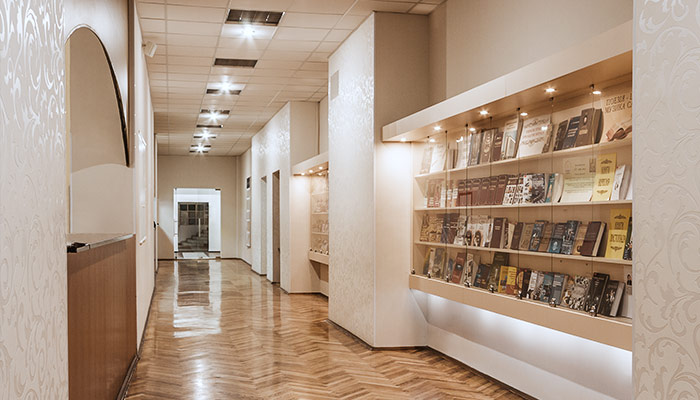
\includegraphics{img/abb_1.jpg}
\caption{Kiev The Main hall - The Library's main hallway}
\end{figure}

\hypertarget{scientific-journal-publishing-process}{%
\section{Scientific Journal Publishing
Process}\label{scientific-journal-publishing-process}}

\hypertarget{stage-1}{%
\subsection{Stage 1}\label{stage-1}}

At first, the field of scholarly journals for arts and culture in
Ukraine was monitored. As a result, the need to create multiple
publishing platforms to present results of unique research on
audiovisual, choreographic, stage, film and television arts, design,
digital communications, etc. was established.

To determine the mission, objectives, readership of potential journals,
a list of researchers as potential authors, editorial boards members and
reviewers was created. We also considered the journals' future role to
make research more visible through the international scientometrics
databases.

When developing the growth and promotion strategy of the publications we
focused at providing the following issues journals require:

\begin{itemize}
\item
  international editorial board and authors,
\item
  standardized name in English,
\item
  the ISSN number for print and online publications,
\item
  digital object identifier (DOI),
\item
  high quality content,
\item
  conclusive English texts and a convincing print design,
\item
  an established publication frequency,
\item
  ethical research standards,
\item
  indexing in bibliographic citation databases, journal lists and
  international search engines.
\end{itemize}

Taking the above into account, it was decided that the main functions of
the newly-established journals should give an idea of the following:

\begin{itemize}
\item
  research trends in Cultural Studies, Art Studies, Social
  Communications that describe major research findings,
\item
  the level of research integration into the global scholarly community,
\item
  the quality of Ukrainian scientific journals of the related subjects,
  in comparison with the international ones,
\item
  publication activity of authors of Ukrainian higher educational
  institutions,
\item
  academic affiliation of scholarly institutions,
\item
  the publications' ranking according to international citation
  databases.
\end{itemize}

\hypertarget{stage-2}{%
\subsection{Stage 2}\label{stage-2}}

At the second stage, in October 2018, the Scientific Library turned into
an active participant of the publishing process and the editorial
support for thirteen scientific publications.

It should be noted that the \enquote{functioning of scholarly publishing
is intended to arrange a well-organised connection between the author,
the editorial board, the editors, the publisher, and the reader. The
effectiveness and success of the journal's work -- its rankings depend
on these links' state of being organised}\footnote{Yulia Didenko and
  Anna Radchenko, \enquote{Publishing activity as a way of scientific
  communication and pursuit of ratings}, \emph{Bulletin of the National
  Academy of Sciences of Ukraine}, 9, (2017): pp.~82--98.
  \url{https://doi.org/10.15407/visn2017.09.082}}. Taking into account
the recommendations of the \enquote{Mohylanskii Protocol}, which states
that \enquote{the owner (founder) of the journal and the editorial staff
are responsible for the journal as a reliable source of high-quality
scientific information on a specific subject}\footnote{Sergei Nazarovets
  and Tatyana Yaroshenko, \enquote{The Mohylanskii Protocol:
  Recommendations for Improving the Editorial Policies of Ukrainian
  Scientific Publications}, \emph{Science of Ukraine in the world
  information space}, 11, (2015): pp.~56--59.}, there are selected chief
editors and members of the editorial boards of scientific journals. The
academic prestige of the scientists, their active profiles in Scopus or
Web of Science and their articles in these citation indices were taken
into consideration.

\begin{figure}
\centering
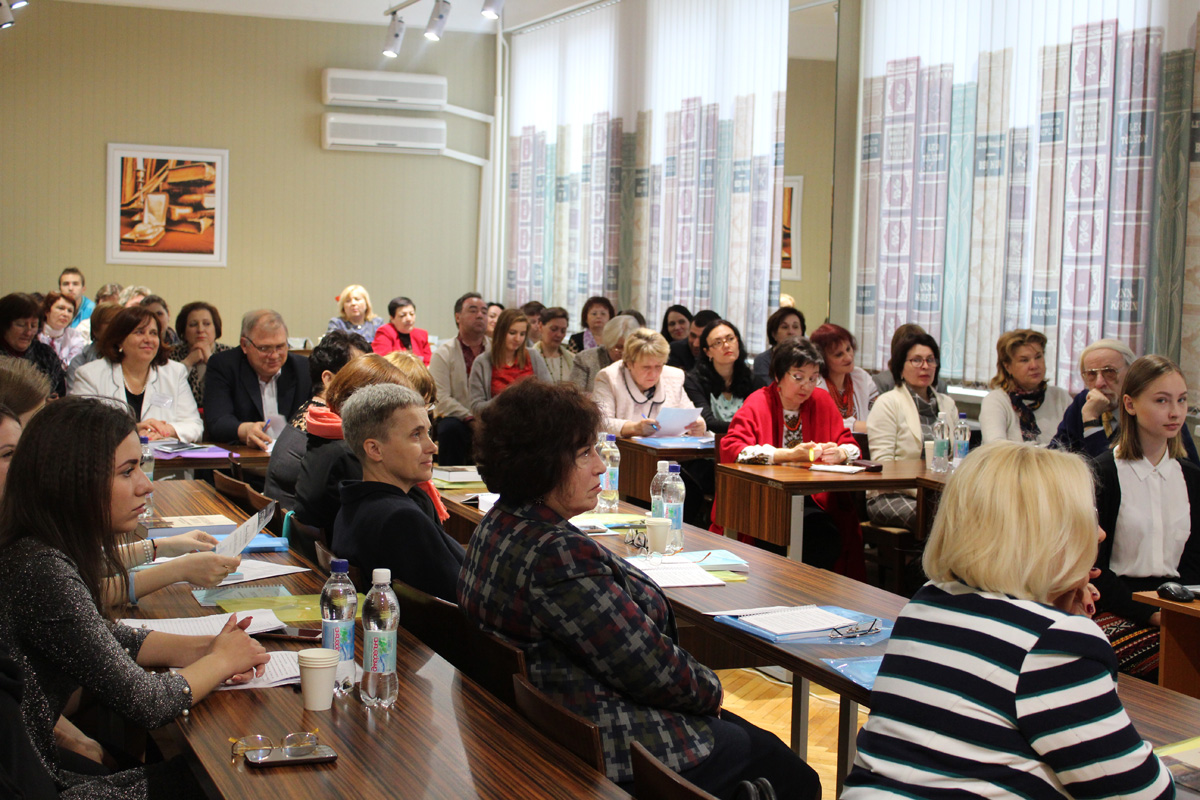
\includegraphics{img/abb_2.jpg}
\caption{Participants of a seminar called Library.Book.Science in 2018}
\end{figure}

\hypertarget{scientific-journals-an-overview}{%
\section{Scientific Journals: An
Overview}\label{scientific-journals-an-overview}}

Six out of the thirteen journals under discussion are subject matter
series of the Bulletin of the Kyiv National University of Culture and
Arts scientific papers collection.

\textbf{\emph{1. \enquote{Bulletin of the Kyiv National University of
Culture and Arts. Series: Audiovisual Art and Production}.}}

Published by: Faculty of Film and Television. Brief description: general
theoretical, artistic, historical, and practical topics on audiovisual
art and production, the results of artists' work studies, archival
researches, and bibliographic reviews\footnote{\emph{Bulletin of the
  Kyiv National University of Culture and Arts}, Series: Audiovisual Art
  and Production, \url{http://audiovisual-art.knukim.edu.ua/}}.

The editorial board: 26 members, of these, 4 are scientists from Kuwait,
Spain, Poland, and Belarus. The editor-in-chief: Alexander Bezruchko,
Doctor of Art Studies, Professor.

\textbf{2. \emph{\enquote{Bulletin of the Kyiv National University of
Culture and Arts. Series in Management of Social and Cultural
Activity}.}}

Published by: Faculty of Event Management, Fashion and Show Business.
Brief description: theory, history, culture and art issues of
management, its socio-cultural achievements and future development in
Ukraine and all over the world. This is a scientific platform designed
to exchange the ideas and share opinions on the development trends of
management in the social and cultural field\footnote{\emph{Bulletin of
  the Kyiv National University of Culture and Arts}, Series in
  Management of Social and Cultural Activity,
  \url{http://sociocultural.knukim.edu.ua/}}.

The editorial board: 24 members, of these, 5 are representatives of the
Netherlands, Poland, Hungary, the USA, and Portugal. The
editor-in-chief: Yaroslav Martynyshyn, Doctor of Economics, Professor.

\textbf{\emph{3. \enquote{Bulletin of the Kyiv National University of
Culture and Arts. Series in Museology and Monumental Studies}.}}

Published by: Faculty of Information Policy and Cybersecurity. Brief
description: theoretical, historical, applied issues of museum studies
and the monument conservation; collective memory, politics of memory;
innovation in the development of museum studies, promoting
them\footnote{\emph{Bulletin of the Kyiv National University of Culture
  and Arts}, Series in Museology and Monumental Studies,
  \url{http://museum-monument.knukim.edu.ua/}}.

The editorial board: 13 scientists, of these, 5 are from Sweden,
Moldova, Poland, Belarus, and Georgia. The editor-in-chief: Serhii
Pustovalov, Doctor of Historical Sciences, Professor.

\textbf{\emph{4. \enquote{Bulletin of the Kyiv National University of
Culture and Arts. Series in Musical Art}.}}

Published by: Faculty of Musical Arts. Brief description: theory and
history issues of Ukrainian and world musicology, theoretical, creative
and methodological problems of the development of musical arts under
contemporary conditions. It covers the results of studies of artists'
work, archival research, and bibliographic reviews\footnote{\emph{Bulletin
  of the Kyiv National University of Culture and Arts}, Series in
  Musical Art, \url{http://musical-art.knukim.edu.ua/}}.

The editorial board: 15 members, of these, 4 represent art scholarly
traditions of Slovenia, Azerbaijan, Australia, and Poland. The
editor-in-chief: Tatiana Humeniuk, Doctor of Philosophy, Professor.

\textbf{\emph{5. \enquote{Bulletin of the Kyiv National University of
Culture and Arts. Series in Stage Art}.}}

Published by: Faculty of Performing Arts. Brief description: theory,
history and practice of world and Ukrainian performing arts\footnote{\emph{Bulletin
  of the Kyiv National University of Culture and Arts}, Series in Stage
  Art, \url{http://artonscene.knukim.edu.ua/}}. The objectives are to
promote the creation of open information space for communication between
leading scientists, young scientists, and experts.

The editorial board: 31 scientists. Of these, 9 are scientists from
Kuwait, Georgia, Belarus, Azerbaijan, Latvia, India, and Lithuania. The
editor-in-chief: Martinas Petrikas, Doctor of Art Studies, Associate
Professor (Republic of Lithuania).

\textbf{\emph{6. \enquote{Bulletin of the Kyiv National University of
Culture and Arts. Series in Tourism}.}}

Published by: Faculty of Tourism, Hotel and Restaurant Business. Brief
description: topical issues on the theory and methodology of tourism,
the scientific backgrounds of tourism for sustainable development, the
key features of the information and innovation activities in tourism and
the management of tourism industry agents, the cultural issues of
tourism development in modern conditions\footnote{\emph{Bulletin of the
  Kyiv National University of Culture and Arts}, Series: Tourism,
  \url{http://tourism.knukim.edu.ua/}}.

The editorial board: 15 members. Foreign schools for science are
represented by scientists from Belarus, Slovakia, and the People's
Republic of China. Chairman of the editorial board is Volodymyr
Antonenko, Doctor of Geographical Sciences, Professor.

\textbf{\emph{7. \enquote{Demiurge: ideas, technologies, perspectives of
design}.}}

Published by: Faculty of Design and Advertising. Brief description:
design development, a platform created for searching models and ways to
solve them. The objectives are to cover the problems of theory, history,
practice and the prospects for the development of design and visual
practices in Ukraine and the world\footnote{\emph{Demiurge},
  \url{http://demiurge.knukim.edu.ua/}}.

The editorial board: 13 members, two of them represent art schools of
Poland and Italy. The editor-in-chief: Liliana Vezhbovska, PhD in Art
Studies, Associate Professor.

\textbf{\emph{8. \enquote{International Relations: Theory and Practical
Aspects}.}}

Published by: Faculty of International Relations. Brief description:
international relations, public communication and regional studies
related to historical and theoretical questions of international
relations; foreign policy and diplomacy; international law; world
economy and international economic relations; public relations and
language support of international activity; social research in the field
of international relations\footnote{\emph{International Relations}:
  Theory and Practical Aspects,
  \url{http://international-relations.knukim.edu.ua/}}.

The editorial board: 17 members, of these, 4 represent foreign academic
schools of Poland and the Czech Republic. The editor-in-chief: Valerii
Lastovsky, Doctor of Historical Sciences, Professor.

\textbf{\emph{9. \enquote{Restaurant and Hotel Consulting.
Innovations}.}}

Published by: Faculty of Tourism, Hotel and Restaurant Business. Brief
description: development of hotel and restaurant business, as follows:
innovative development of hotel and restaurant places; current issues of
culinology, enogastronomy, anthropology of food and serviceology; theory
and practical aspects of the food technologies of functional purpose
adoption; the issues regarding the food ecology and hotel and catering
services; economy, marketing, management, competitiveness, modern IT
solutions within the hotel and restaurant business. The publication aims
to advance scientific studies in hotel and restaurant
business\footnote{\emph{Restaurant and Hotel Consulting. Innovations},
  \url{http://restaurant-hotel.knukim.edu.ua/}}.

The editorial board: 22 scientists, 6 of them represent institutions of
science in Poland, Sweden, Azerbaijan, Turkey, USA, and Bulgaria. The
editor-in-chief: Hryhorii Deynichenko, Doctor of Technical Sciences,
Professor.

\textbf{\emph{10. \enquote{Dance Studies}.}}

Published by: Faculty of Choreographic Arts. Brief description: theory,
history and practice of Ukrainian and international choreographic
culture; interdisciplinary issues regarding the choreography\footnote{\emph{Dance
  Studies,} \url{http://dancestudios.knukim.edu.ua/}}.

The editorial board: 14 members, 4 of them represent dance schools of
Spain, Belarus, Slovakia, and the USA. The editor-in-chief: Olexander
Chepalov, Doctor of Art Studies, Professor.

\textbf{\emph{11. \enquote{Ukrainian Journal of Library and Information
Sciences}.}}

Published by: Faculty of Information Policy and Cybersecurity.

Brief description: theory and applied aspects of library science,
bibliography, archive science, document science, information technology,
information, library and archive practices\footnote{\emph{Ukrainian
  Journal of Library and Information Sciences},
  \url{http://librinfosciences.knukim.edu.ua/}}.

The editorial board: 15 members, 5 of them are representatives of
institutions of the science of Belarus, the USA, and Poland. The
editor-in-chief is Tatiana Hranchak, Doctor of Social Communications,
Senior Researcher.

\textbf{\emph{12. \enquote{Ukrainian Information Space}.}}

Published by: Faculty of International Relations and Journalism. Brief
description: the analysis of development and activity practice of the
Ukrainian information space in social and political realities of Ukraine
and within the world context; theory, practical and historical aspects
of the main components of the Ukrainian information space: press, radio
and TV broadcast, online platforms and printed editions\footnote{\emph{Ukrainian
  Information Space,} \url{http://ukrinfospace.knukim.edu.ua/}}.

The editorial board: 16 scientists, 4 of them are representatives of
institutions of the science of Lithuania, Poland, and the USA. The
editor-in-chief: Mykola Tymoshyk, Doctor of Philology, Professor.

\textbf{\emph{13. \enquote{Digital Platform: Information Technologies in
the Sociocultural Sphere}.}}

Published by: Faculty of Information Policy and Cybersecurity. Brief
description: theory and applied aspects of information technology,
computer science, graphic visualization, information and communication
technologies in the socio-cultural sphere\footnote{\emph{Digital
  platform}: information technologies in sociocultural sphere,
  \url{http://infotech-soccult.knukim.edu.ua/}}.

The editorial board: 11 members, including representatives of schools
for the science of Bulgaria, Austria, and Lithuania. The
editor-in-chief: Ata Ovezgheldyev, Doctor of Engineering Science.

The frequency of issues in all journals is twice a year (June,
December). All materials are distributed under a Creative Commons
Attribution 4.0 International License. The authors retain copyright and
publication rights without limitation.

\hypertarget{collaboration-with-editorial-boards}{%
\subsection{Collaboration with editorial
boards}\label{collaboration-with-editorial-boards}}

Collaborating with the editorial boards of the journals between 2018 and
2019, the library undertook the work of obtaining the publications' ISSN
(each for print and online) and ISSN ID certificates in the
International Centre (France).

To ease the findability of scholarly publications within a wide range of
scientific databases, there is an assignment procedure of DOI for the
articles. As of 2020, all articles of periodical publications of the
University have a DOI.

Since a key element of a new scientific publication promotion is an
informative and well-designed website, which is a journal's landmark in
e-science space, the IT department of the Scientific Library created and
managed the website for each edition using Open Journal Systems (OJS).
This includes metadata publishing of journal articles, homepage
preparation of the journal issues, integrity ensuring of the database
and the landing pages of the scientific journals and regular backup
copies.

There is a support service to provide the scientific editorial staff and
authors with full tutorial instructions on how to use OJS. It
coordinates efforts and unifies the editorial policy of all thirteen
journals.

The websites of the journals currently use an Open Journal Systems
2.4.4.1 open-source software package, which serves the processes of
management and publication. The package is developed, maintained, and
distributed for free by the Public Knowledge Project under the GNU
General Public License.\footnote{\url{https://pkp.sfu.ca/ojs/}}

\hypertarget{stage-3.-indexing-in-international-databases}{%
\subsection{Stage 3. Indexing in international
databases}\label{stage-3.-indexing-in-international-databases}}

In 2018, we began to integrate the new university journals into
international databases and reference lists. This process lasted in 2019
as well. Now, all scientific journals and collections of scientific
papers are indexed in Crossref cross-publisher reference, in search
engines and the databases of BASE, Google Academy, Central and East
European Index, WorldCat and in the \enquote{Scientific Periodicals of
Ukraine} information resource by the Vernadsky National Library of
Ukraine.

All journals are indexed in the international databases of Academic
Resource Index (ResearchBib), Index Copernicus Journals Master
List\footnote{\url{https://indexcopernicus.com/index.php/en/parametryzacja-menu-2/journals-master-list-2}},
Polska Bibliografia Naukowa (but \enquote{International Relations:
Theory and Practical Aspects}).

The journal \enquote{Ukrainian Information Space} is additionally
presented on the research portal ResearchGate.

The scientific journals' websites are placed on the platform of the
Ukrainian research and academic network URAN, Directory of Open Access
Journals (DOAJ), one of the most famous search services in the world
that provides information to open access materials and indexes both
journal and scientific article titles; as well as on Ulrichsweb
(Ulrich's Periodicals Directory), an authoritative international
database of periodicals.

\hypertarget{future-stages}{%
\subsection{Future stages}\label{future-stages}}

In the future, to promote the University's scholarly publications in
prestigious databases, lists and search engines, the library will
provide training and workshop sessions for authors of articles. The
program includes lessons on how to write abstracts, on shifting to
e-publishing system-based networking between the author and journal
team; to train authors basic principles of using digital article
preparation tools offered by Scopus and Web of Science and therefore
also to use Mendeley and EndNote.

An important task will be the development of the system into open access
defined by the Budapest Open Access Initiative (BOAI, Budapest Open
Access Initiative) via:

\begin{itemize}
\item
  participation of the University's scientists in international projects
  of scientific communication,
\item
  registration of the university's repository in international search
  engines,
\item
  listing of all scientific journals of the University in open access
  directories,
\item
  articles' compliance with the requirements of scientometrics databases
  (peer-reviewed, English language, with structured abstract, references
  and relevant metadata).
\end{itemize}

\begin{figure}
\centering
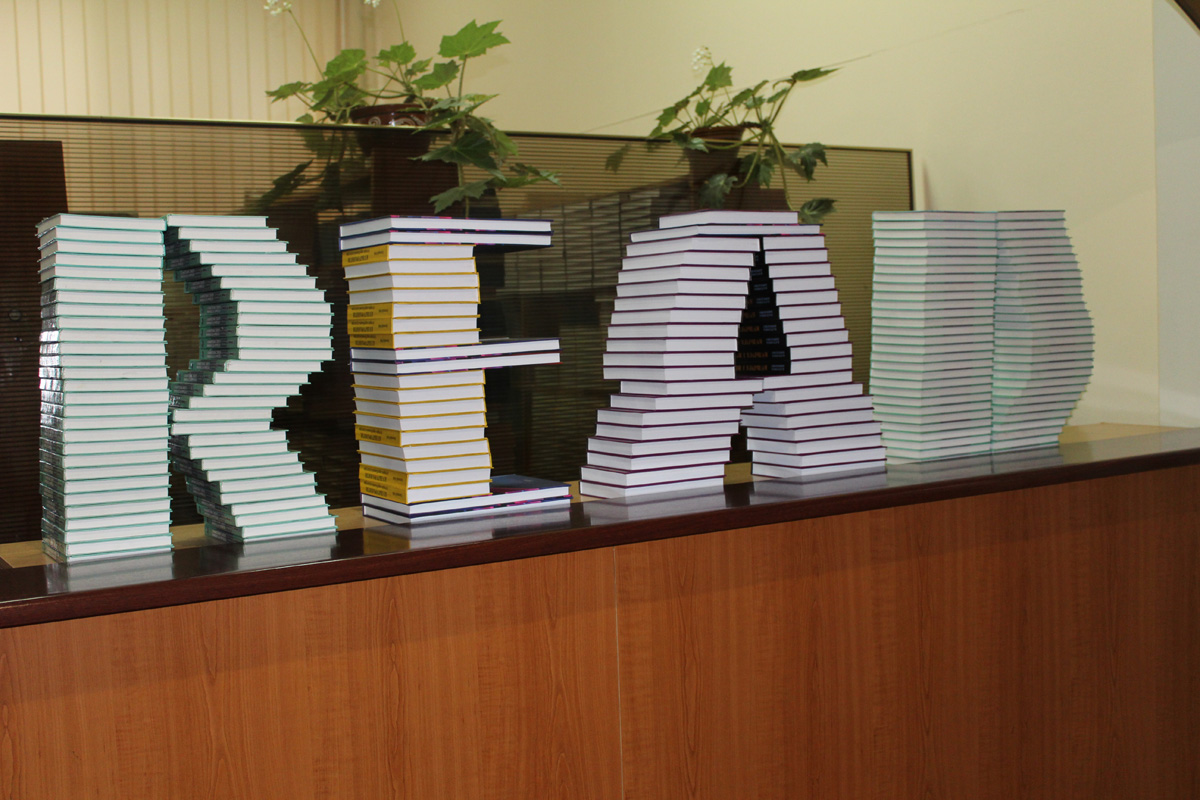
\includegraphics{img/abb_3}
\caption{Installation near the library's checkpoint}
\end{figure}

\hypertarget{conclusions}{%
\section{Conclusions}\label{conclusions}}

Thus, the Scientific Library of the Kyiv National University of Culture
and Arts is completing a complex process of redesigning its role and
tasks within the system of scientific communication of the University.

The article has presented the library's contribution to the editorial
and publishing process, as well as to the promotion of thirteen new
scientific journals of the University. It has provided a description of
the mission, objectives of scientific publications, editorial staff,
stages and promotion results within the international databases and
lists.

Looking ahead, the Scientific Library's activity will be focused on the
development of information-analytical monitoring and bibliometric
analysis of communication systems of the University; a design for the
representation of scientists' profiles in the search engines and the
international scientometrics databases; facilitating the indexing of
scientific journals of the University in Scopus and Web of Science as
international databases.

Priorities include the support of e-publishing and the development of
individual awareness of lecturers for scholarly research based on
international scholarly resources.

Providing the scientific and educational work with information support,
the library transforms its role and objectives, reinventing itself from
the auxiliary research element to an active participant of scientific
and educational work. It boosts the scientific ranking of institutions
of higher education and researchers' brand names as well.

%autor
\begin{center}\rule{0.5\linewidth}{0.5pt}\end{center}

\textbf{Yurii Horban}, PhD in Cultural Studies, Associate Professor,
Scientific Library, Director. Kyiv National University~of Culture and
Arts, 36, Yevhena Konovaltsia St., Kyiv, 01133, Ukraine. E-mail:
y.i.gorban@gmail.com. ORCID: 0000-0001-5837-4409.

\textbf{Viacheslav Lukianenko}, Scientific Library, Head of IT
Department. Kyiv National University~of Culture and Arts, 36, Yevhena
Konovaltsia St., Kyiv, 01133, Ukraine. E-mail:
vyacheslav.lukyanenko@gmail.com. ORCID: 0000-0002-6519-1253

\textbf{Olena Skachenko}, Scientific Library, Head of Sector. Kyiv
National University~of Culture and Arts, 36, Yevhena Konovaltsia St.,
Kyiv, 01133, Ukraine. E-mail skachenko.nana@gmail.com. ORCID:
0000-0003-3827-5985

\end{document}
